% Author : Alain Matthes
% Source : http://altermundus.com/pages/examples.html
\documentclass[12pt]{article}

\usepackage[utf8]{inputenc}
\usepackage[upright]{fourier}
\usepackage{tikz}
\usetikzlibrary{matrix,arrows,decorations.pathmorphing}
\usepackage{verbatim}

\begin{comment}
:Title: Matrix multiplication
:Use page: 1

Illustration of how to compute the product of two matrices.

:Source: `Altermundus.com`_

.. _Altermundus.com: http://altermundus.com/pages/examples.html
\end{comment}

\begin{document}



%To multiply two matrices, the first matrix must have the same number of rows (p) as the second matrix has columns (q).  In other words, p of the first matrix must equal q of the second matrix. In general terms, a matrix C which is a product of two matrices, A and B, will have elements given by the following 
%\[c_{ij}=\sum_{k=1}^p a_{ik}b_{kj}\]
% where $i$ = ith row and $j$ = jth column


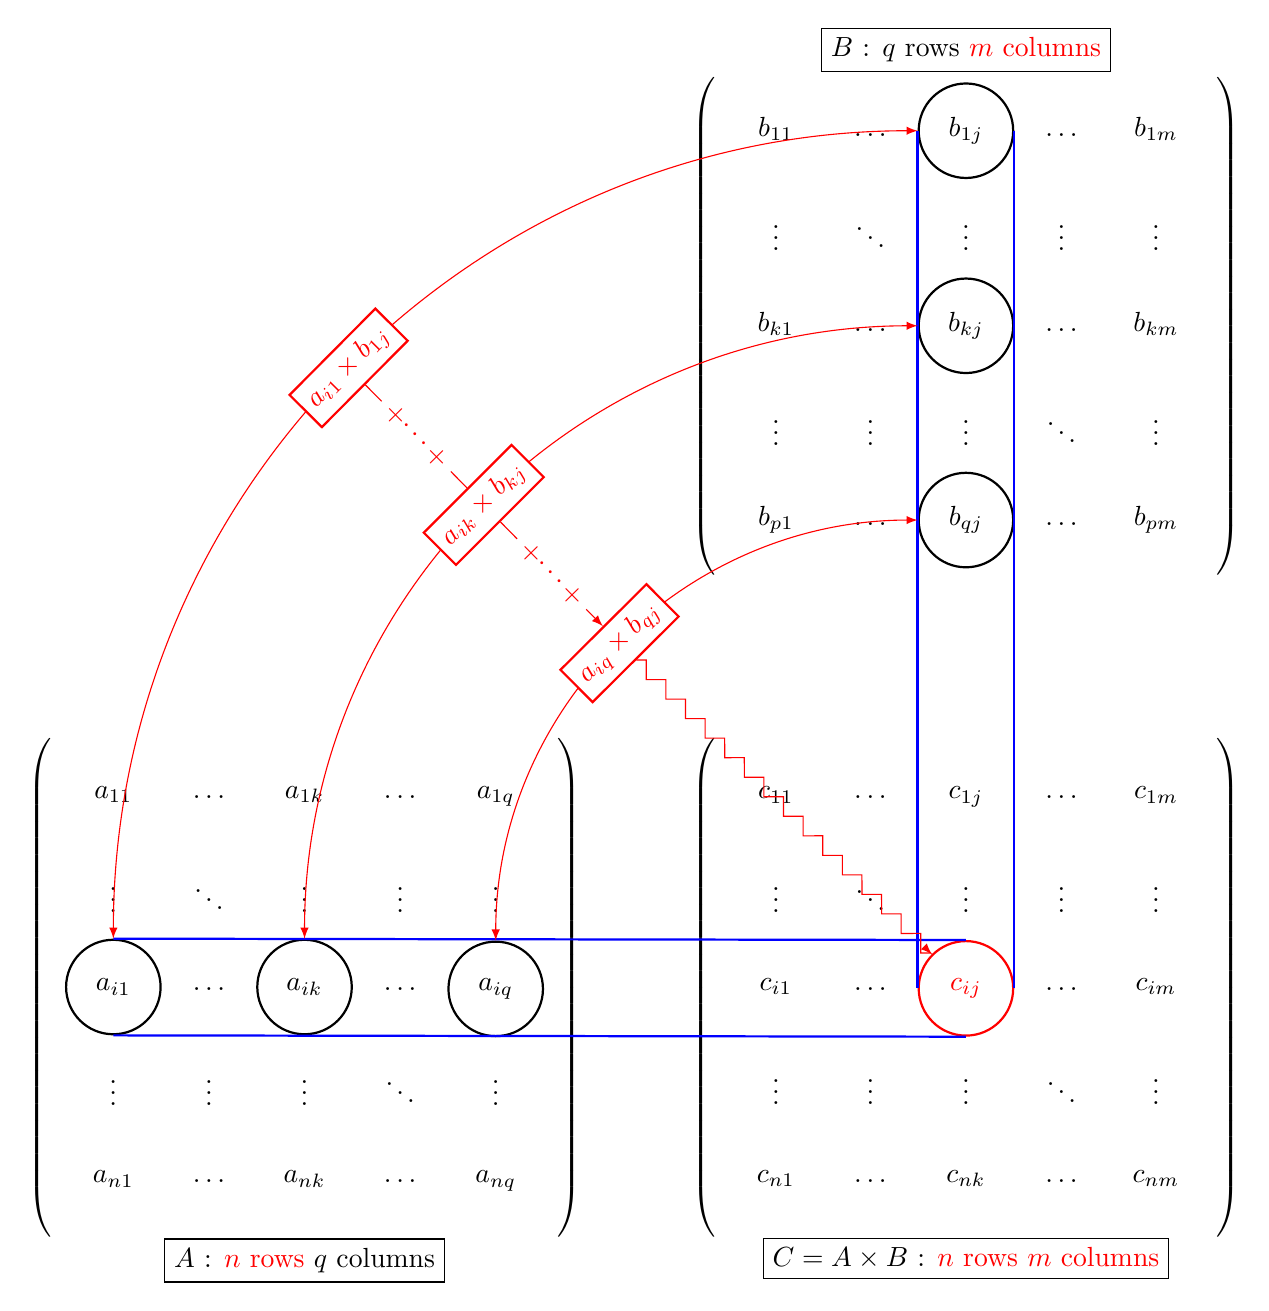
\begin{tikzpicture}[>=latex]
% unit
\newcommand{\myunit}{1.2 cm}
% the styles
\tikzset{node style sp/.style={draw,circle,minimum size=\myunit,thick}}  
\tikzset{node style ge/.style={circle,minimum size=\myunit}}
\tikzset{arrow style mul/.style={draw,sloped,midway,fill=white,thick}}
\tikzset{arrow style plus/.style={midway,sloped,fill=white,thick}}
% defintion of matrices
\matrix (A) [matrix of math nodes,%
             nodes = {node style ge},%
             left delimiter  = (,%
             right delimiter = )] at (0,0)
{%
  a_{11} &\ldots & a_{1k} & \ldots & a_{1q}  \\ 
    \vdots & \ddots & \vdots & \vdots & \vdots \\
  |[node style sp]|{a_{i1}}& \ldots%
         & |[node style sp]| {a_{ik}}%
                  & \ldots%
                           & |[node style sp]| {a_{iq}} \\ 
  \vdots & \vdots& \vdots & \ddots & \vdots  \\
  a_{n1}& \ldots & a_{nk} & \ldots & a_{nq}  \\ 
}; 
\node [draw,below] at (A.south) { $A$ : \textcolor{red}{$n$ rows} $q$ columns};
\matrix (B) [matrix of math nodes,%
             nodes = {node style ge},%
             left delimiter  = (,%
             right delimiter =)] at (7*\myunit,7*\myunit)
{% 
  b_{11} &  \ldots& |[node style sp]| {b_{1j}}%
                  & \ldots & b_{1m}  \\ 
  \vdots& \ddots & \vdots & \vdots & \vdots \\
  b_{k1} &  \ldots& |[node style sp]| {b_{kj}}%
                  & \ldots & b_{km}  \\ 
  \vdots& \vdots & \vdots & \ddots & \vdots \\
  b_{p1} &  \ldots& |[node style sp]| {b_{qj}}%
                  & \ldots & b_{pm}  \\ 
};
\node [draw,above] at (B.north) { $B$ : $q$ rows \textcolor{red}{$m$ columns}}; 
% matrice résultat
\matrix (C) [matrix of math nodes,%
             nodes = {node style ge},%
             left delimiter  = (,%
             right delimiter = )] at (7*\myunit,0)
{% 
  c_{11} & \ldots& c_{1j} & \ldots & c_{1m} \\ 
  \vdots& \ddots & \vdots & \vdots & \vdots \\
    c_{i1}& \ldots & |[node style sp,red]| {c_{ij}}%
                  & \ldots & c_{im} \\ 
  \vdots& \vdots & \vdots & \ddots & \vdots \\
  c_{n1}& \ldots & c_{nk} & \ldots & c_{nm} \\ 
}; 
\node [draw,below] at (C.south) {$ C=A\times B$ : \textcolor{red}{$n$ rows}  \textcolor{red}{$m$ columns}};
% arrows
\draw[blue,thick] (A-3-1.north) -- (C-3-3.north);
\draw[blue,thick] (A-3-1.south) -- (C-3-3.south);
\draw[blue,thick] (B-1-3.west)  -- (C-3-3.west);
\draw[blue,thick] (B-1-3.east)  -- (C-3-3.east);
\draw[<->,red](A-3-1) to[in=180,out=90] 
    node[arrow style mul] (x) {$a_{i1}\times b_{1j}$} (B-1-3);
\draw[<->,red](A-3-3) to[in=180,out=90] 
    node[arrow style mul] (y) {$a_{ik}\times b_{kj}$}(B-3-3);
\draw[<->,red](A-3-5) to[in=180,out=90] 
    node[arrow style mul] (z) {$a_{iq}\times b_{qj}$}(B-5-3);
\draw[red,->] (x) to node[arrow style plus] {$+\raisebox{.5ex}{\ldots}+$} (y)%
                  to node[arrow style plus] {$+\raisebox{.5ex}{\ldots}+$} (z);  
\draw[->,red,decorate,decoration=zigzag] (z) -- (C-3-3.north west);
\end{tikzpicture} 
\end{document}
 
% encoding : utf8
% format   : pdfLaTeX
% author   : Alain Matthes